\chapter{Methodology} 
\label{ChapterMeth}
\largerpage

\begin{sloppypar}
This chapter provides meta-information on our data collection, that is, that of the work group and me. It gives an overview of the methods used by us to gather the data discussed in the book. This includes the methods and thematic foci of data elicitation, the speakers we worked with in general and who the main consultants were, as well as some notes on climate and culture.
\end{sloppypar}

%\section{Methods}
\label{sec:Meth}

%Who the consultants were and their linguistic backgrounds and where they’re from in relation to all the stuff we already talked about and how great that whole thing was to be with them and  ... 


%In terms of educational background, I completed my MA in Language Documentation and Description at SOAS in December 2016. Along with a fieldwork class in Bern, the MA gave me a solid foundation and almost two years of experience in working with language data and speakers. In Bern and at SOAS, I had theoretical classes on linguistic, anthropological and methodological subjects.% I am familiar with the software I will use, with techniques of audio and video recording, and was sensitised to issues of usability and transparent data management. During this time, I have had the opportunity of working with all major types of recording equipment and to familiarize myself with the contexts in which to use them.
%The fieldwork course let me acquire theoretical knowledge and practical skills related to obtaining and analysing linguistic data. The courses involved designing, conducting and recording elicitation sessions with research participants, compiling a lexical
%database (in Toolbox and in FLEx), grammatical annotation through FLEx and ELAN (including morpheme-by-morpheme glossing), and finally translation of the data, as well as describing aspects of phonology, morphology and syntax of a language I was previously unfamiliar with. I am in grateful debt to my teachers. 
\section{Types of data recorded}

While the author hopes that this will not be the last work done on the language, this work attempts to give as comprehensive a description as possible. Since this may well be the last record of the language, and in any case the only one of Vamale as spoken in this period, the usability of the data is crucial. The work group recorded as much as possible, with members of every clan, spanning every generation but the youngest, and both genders (though a focus on males was hard to avoid for cultural reasons). We made videos of ceremonies, everyday activities, in Vamale as well as in other languages, and still missed hunts, funerals, and a women's craft week. The work group usually met three times a week and spent the entire day together. The days in between were spent transcribing and annotating, as well as preparing the next session. The elicitation sessions were usually structured in the following way: once the date, speaker, and location had been recorded, consent was established, and an overview of the topics of the day was given, in case a consultant wanted to avoid a certain topic. While the interviews with members of the local clans were conducted in Vamale as much as possible to avoid priming, the elicitation sessions with the work group most often featured questions and discussions in French, and answers in Vamale. Coffee, tobacco and food were provided by the researcher, along with customary gifts when meeting a consultant for the first time.

Data from transcribed data incorporated into FLEx carries references in the format L(L)(N):NN(N), e.g. KL:126, where the first part designates the text in the FLEx database, and the second the line number. Other data either shows the title of the audio recording and the time signature of the utterance, or the date and page of the notebook entry. Some data was overheard or so frequently used that no reference was given. 
%Most of this material remains untranscribed, and some recordings were not made due to fatigue of the researcher. Transcription, though initially planned to happen in the field, was mostly done in Bern using ELAN and FLEx. Description-wise, major gaps remain on prosody, and the semantics of some constructions. 

As explained in other sections (\sectref{ssec:Frenchpolicy}, \sectref{sec:Multiling}), there are few villages in the area that speak a single language, and Vamale is spoken exclusively in multilingual environments. French dominates in most places, but even where most people communicate in Oceanic languages, Vamale is almost never the majority language. This complex sociolinguistic situation is one reason for the relatively long period spent in the field, as every clan idiolect was recorded. The recordings are all marked for the speakers and place involved, leaving material for future research on language variation. 
A simple dictionary was compiled in the field using \citegen{leenhardt_langues_1946} wordlist and existing dictionaries of other languages as prompts, as well as the recorded data. Priming and misunderstandings were unavoidable, and language attrition contributed to the difficulties. Several elicitation sessions were dedicated to cross-checking this data and illustrating it with example sentences, and elders were visited explicitly to check old words. All materials are open-access and available online via the Endangered Languages Archive (ELAR), \href{https://elar.soas.ac.uk/Record/MPI1282765}{collection 0470}. The recorded data is also stored in the Archive of the Northern Province in Hienghène, as well as on SD cards left with the respective speakers. 

\section{Equipment used}
The project used the following equipment:

\begin{itemize} 
	\item Sennheiser headphones HD201, with a splitter to listen to recordings in groups
	\item Røde NTG-2 super-cardioid ``shotgun" microphone (a dead cat is appropriate on the coast due to the winds), and a Sennheiser EW122 lavalier microphone.
	\item a Canon XA30 camera, which can record audio in .wav format, has a powerful visual zoom, but a weak battery
	\item a Zoom H6 recorder
\end{itemize}

\section{Field trips}
A first field trip was undertaken in 2016, chiefly to ask for permission and support in the speaker area and from the relevant organizations: the Academy of Kanak Languages, the University of Nouméa, and the local customary authorities. This took two weeks, during which first lexicographical data were gathered. The research in 2017 lasted a little over 5 months, between June and December, the dry season. The first major stay was dedicated to gathering data from every speaker clan, and to do so in the form of stories and life recollections, as this was important to legitimize the project in the eyes of the speaker communities. The interviews were usually public, and several people would sit, listen, and occasionally chime in. I often mixed grammatical elicitation with text production, i.e. the first part would ask the consultants to check prepared sentences in Vamale or translate French ones, and the second part would invite them to speak about what they wanted. The latter part often revolved around the societal changes that occurred in their lifetimes, but some also commented on climate change, or narrated oral history. Most of these interviews were filmed as well, depending on the consent given (however, the camera battery gave out more than once in the first year). I also gathered botanical and zoological data and filmed people gardening and fishing, as well as building roofs and boats. Whenever possible, I participated in the activities I documented. The second field trip in 2018, around four months long, shifted the focus more to elicitation sessions, as the Bwatoo, Nêlêmwa, and Cèmuhî grammars were used as reference points to identify gaps in the description of Vamale. A third trip in 2019 focused on filling gaps, handing over data to the respective speakers (on SD cards, which was useless as most lack access to card readers; will be done differently next time), and transcribing as much as possible of the data gathered in the previous years. 

%rewrite the following. 

%

%The biggest villages, with an overall population of around 250, are Thewaade / Tiouandé, Thenganepaik / Téganpaik, and Wanaa / Ouanache. This is where most of the research took place, as it can take hours to the more remote settlements, and the roads are unreliable during rainy periods. 
%I budgeted enough SD-cards to be able to leave the data on them once recorded, thus already creating a card library. SSD harddrive disks will also receive the data as backup, and
Because of the amount of data recorded, time in the field did not allow for a complete transcription of the recordings. In order to alleviate the task, the author attempted to hire and train two locals to help him transcribe. This did not succeed as people were not used to sitting for hours, nor to working with computers. The most useful technique was to ask people to listen to the recording and repeat it clearly word for word for him to write down. This was particularly effective for the recordings of elders who were difficult to understand.

\section{Consultants} 
\label{sec:Consultants}
%This is how we will deal with this controversy and how we will name things in this volume which leads into discussion about ...Who the consultants were and their linguistic backgrounds and where they’re from in relation to all the stuff we already talked about and how great that whole thing was to be with them and 

Working on Vamale meant finding speakers willing to work with the researcher for free (except for transcriptions), in order to perpetuate the local custom initiated by French researchers. In exchange, consultants and speakers were welcome to discuss the goals of the project and change them. The project was assigned a team of three motivated representatives of the most powerful local clans. %Three friends of Dui 
Apart from the crucial fact that they had the time and the motivation to do it, they each had a different array of languages and social relations, which was very useful. From this nucleus grew a loose team of speakers joining in. The team members had lives and priorities of their own, and the group's makeup changed several times over the three stays. %This was partly tied to alcohol and personal problems on their side, a lack of cultural understanding on mine, and differences in our goals.

This section says a few words about the four main consultants. My deepest gratitude belongs to all of them. Other important people were Mr.\ Baptiste Ucian who kick-started the lexicon and most of the first months' elicitations, Mrs.\ Elise Kalène who gave a lot of her time to elucidate phonemes, and the entire population of the villages who were happy to share their views on the world, answer spontaneous questions, and always sympathetically asked how the work was going. 

\subsection{André Nigai Kalène}
Mr.\ Kalène is the eldest brother of Tiouandé's chieftain and grew up bilingual in Pije and Vamale. Extremely knowledgeable in traditions and a skillful boat- and house-builder, he was the most patient and reliable consultant and, in the beginning, walked an hour every day to our meetings. He has been politically invested in protecting indigenous rights his entire life. His extensive family network helped us tremendously.

\subsection{Christophe Keela Pei}

Mr.\ Pei is the herald of the powerful Pei clan, which housed and fed the author for ten months. Except for French, Mr.\ Pei is one of the rare monolingual speakers of Vamale, which helped decide whether a word was Vamale or a loan. Mr.\ Pei is a master fisherman and hunter. We often gathered at his house during the first research period.

\subsection{Jacob Keela Ganap Oué}

Mr.\ Oué is the eldest man in the land-owning clan of Wanaa and knows much about traditions, land ownership, and local history. A passionate gardener and ecologist, Mr.\ Oué spent time with Mr.\ Kalène rehabilitating mangroves, and is very knowledgeable about plants and animals. We spent most of our elicitations sessions at his house and he hosted the author for the last month. Mr.\ Oué speaks Vamale, Pije, and Fwâi, as well as excellent French. 

\begin{figure}
	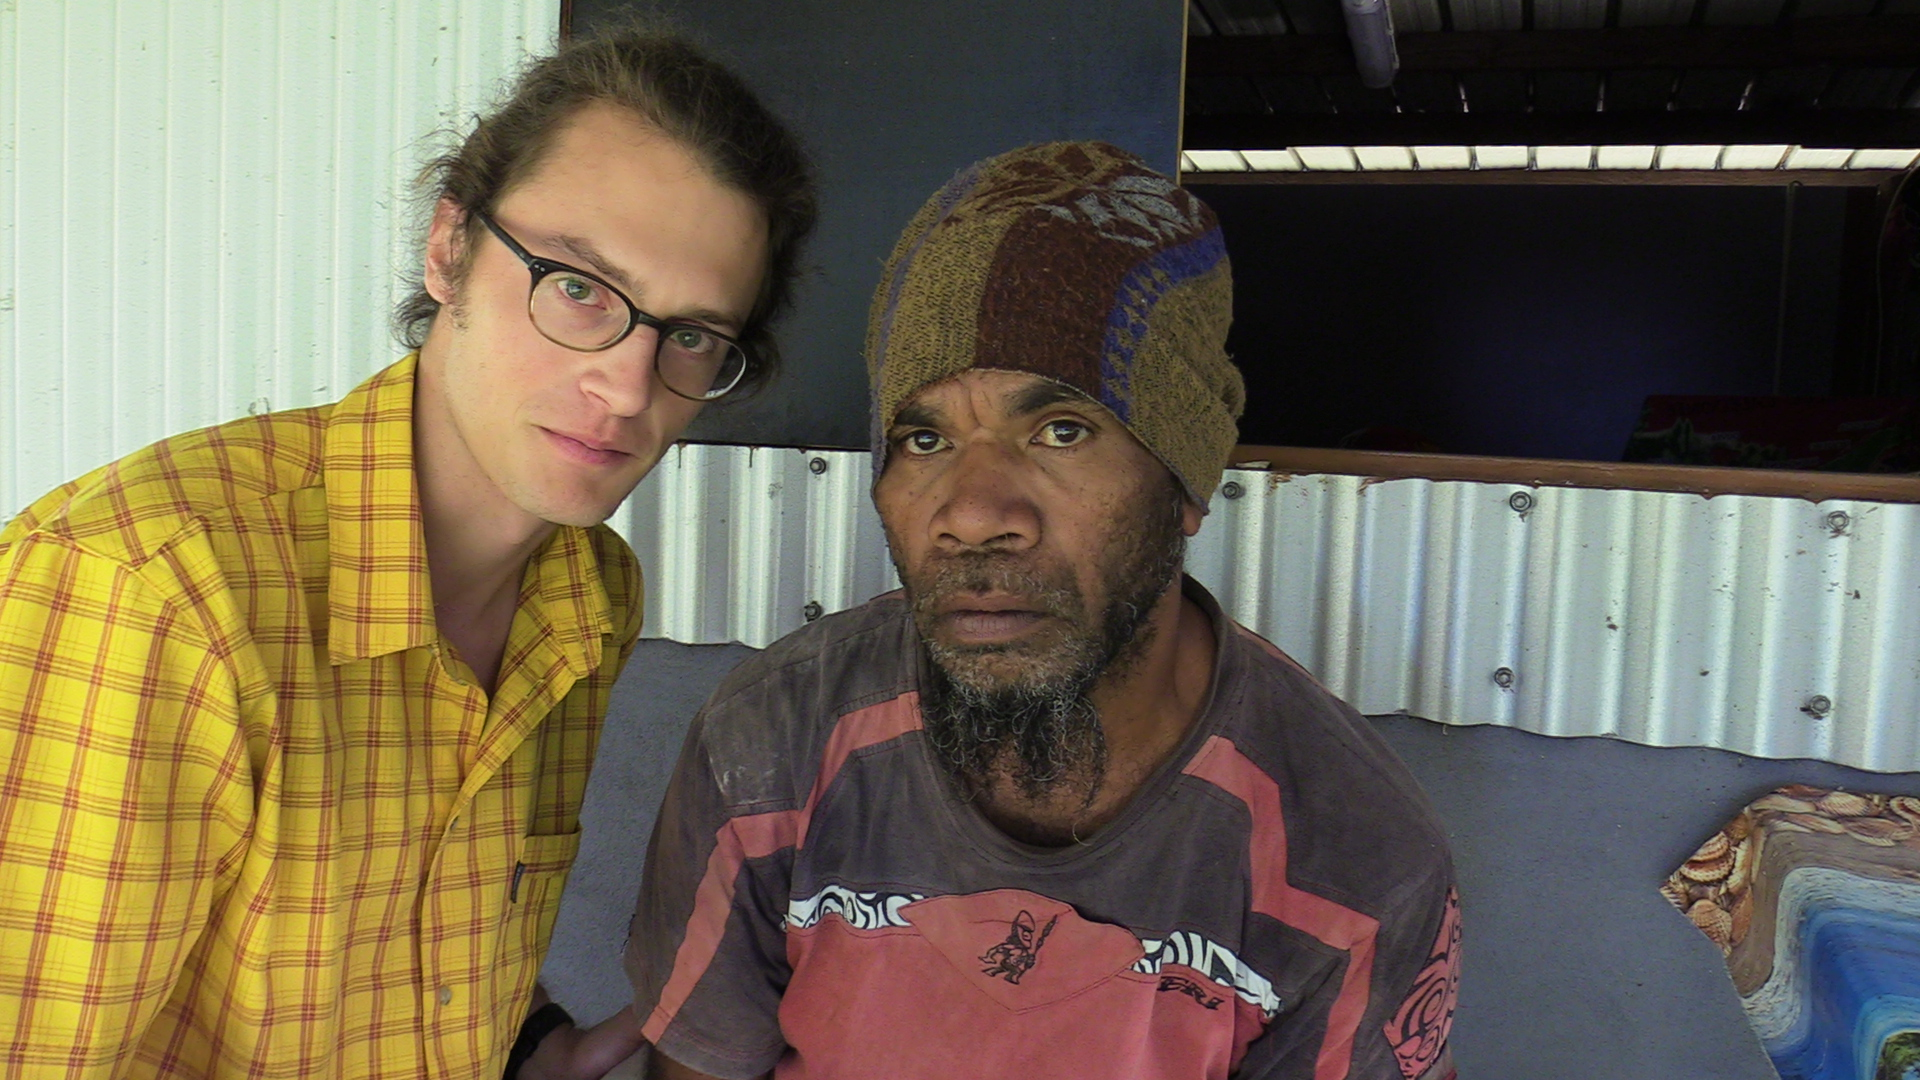
\includegraphics[width=\linewidth]{figures/gana}
	\caption{Mr.\ Jacob Oué and the author}
\end{figure}

\subsection{Jean-Philippe Emyl Téin Oué}

Mr.\ Oué was the only one in the group who was the author's age, and we spent a lot of time together in his garden, at his house, in his woods, and driving around. A speaker of Vamale, and able to understand Pije and Fwâi, he was the consultant most interested in syntax, morphology, and semantics, and spent many patient hours working on transcriptions, subtle differences between morphemes, and phonological questions.

The four men mentioned here guided the work through unspoken customs and laws, taught the author Vamale, and poured their time and hearts into the project. Without their help, most speakers would not have spoken to the author, nor would he have known where to go, and very little would have seen the light of day. \textit{Holeke thuan nyakoovwe ka gavwe i vaaya!}



\section{Notes on fieldwork in Vamale country}
\label{sec:Field}
%This section will refer to \Cref{ChapterContext} and \Cref{sec:Meth}, but does not seem redundant. While 
This work is a linguistic contribution, but some anthropological information is relevant for the reader to understand the cultural context in which the language is embedded, and some hints for future researchers may be useful. The northern east coast of New Caledonia is over 90\% ethnically Kanak, and everyday life is very much defined by this fact. % is not the easiest terrain to work in, and the culture is very different. %While this section try to avoid illusions about the interest of foreigners in working on this language, I hope that the following words will help anyone interested in working in the area, as well as shed some light on the problems I encountered.
%\subsubsection{2016, a sweating idiot.}
%This is a first description of the period between early November and mid-November 2016, which I spent with my then-partner Martha Amy Rose Newman in Téganpaïk. I am writing this from memory and it shall serve as a basis for a later section to be used in the dissertation.
%The east coast of Kanaky is a rainy, humid, warm area. %Grandma's digital watch has a broken thermometer that keeps claiming 30°C+ but it must be around 27-29°C. 
\subsection{Climate}
Although the temperature is relatively stable between 23°C and 28°C, humidity and sudden, unpredictable rain (even more so with climate change) can be dangerous for electronic equipment. The project used waterproof bags and silica gel packs to protect the equipment from humidity, and Lavaliers and hyper-directional microphones to mitigate the noise of the rain. Many roads become difficult when it rains, and most houses are tin-roofed, making recordings inside difficult due to echoes and rain/sticks falling on the roof. Noise from cars driving by on the main road was an almost unavoidable problem for recordings, though chickens took over that role wherever the setting was rural enough to exclude traffic.

%it is beyond me how people can walk for hours in the sun, a t-shirt wrapped around their head, or how they can play football. %I sweat. 
When it rains, it does so violently, and sometimes for days on end, with brief interludes. Tap water becomes murky, then brown, and finally stops working, so water-purifying pills are useful. Electricity may stop working if trees fall on the power lines. %A bucket fills in an hour. When it does not rain, it can remain dry for weeks. 
Because of the powerful weather, the obligation to attend ceremonies (especially unforeseeable funerals), the difficulty of planning an appointment etc., it is advisable to carry recording equipment at all times and record whenever possible, and to understand that plans can change at short notice. Life moves slowly, and people prefer to finish a thing properly to strictly adhering to an appointment. It may be frustrating to consultants to interrupt an interview, so it seemed preferable to keep the day planning flexible instead of \qu{making the most of it} and seeing three consultants in one day. 
% You never know when you meet a person again. % I prefer when it does not rain. Fish everywhere. Loris. Flowers that people in Europe would kill to be able to grow. Mangoes galore. Coconuts. Poingo bananas. 

\subsection{Lodging}
%Téganpaik is the home of Daniel Doui Péi, who worked at the city hall in Touho and thus became the first contact in the field. He housed the author and his partner on the first, exploratory trip in 2016, and later 
The author rented a small house from his first contact and stayed there for most of his time in the area. With the exception of old bachelors and widowers, the researcher was the only person in the village who had a house to themselves, slept alone in a room, and could retire to work whenever needed. On the other hand, this also alienated the author from the others and prolonged the time it took him to integrate into the community. It took approximately six weeks for the shyness to subside on both sides. The author still recommends individual housing, if at all possible. Participating in as many activities as possible helps bridge the gap between the community and the stranger, as recommended by Patience Epps for fieldwork in Hup country \parencite[37]{epps08hup}. %Dui's family fed him for most of his stay. 
Be aware of your imposition on a family, contribute in food and money so as to alleviate the burden you represent. Spend free, disinterested time with your consultants and family, as purely professional relationships hardly exist in a tribal setting. %(it is also nicer to be treated like a friend rather than an employer, boarder, etc).

People usually keep a Spartan interior, with little furniture except for beds, TVs, and an occasional table. Mostly, meals take place outside, where the kitchen tends to be located. In general, most people have little to no disposable income. Most families rely on the employment of a family member as well as their own gardens for subsistence. Customary ceremonies are a major part of life, and exchanging produce, clothing, and money in this context has a function of leveling inequalities: some people can only contribute bananas or fruit bats, but leave a ceremony with clothing, money and sugar. %Coming in with expensive equipment and being white makes one a potential source of revenue, which partly defines most relationships with locals. The author suggests acknowledging this by determining a budget that can be spent for others, and spending it light-heartedly.


%----------------------------------------------------------------------------------------
%	SECTION 2
%----------------------------------------------------------------------------------------

Some anthropological information is relevant to the reader. The northern East Coast of New Caledonia, uncontested \textit{Kanaky}, is not the easiest terrain to work in, and the culture is very different from Western contexts. I hope that the following words will help anyone interested in working in the area, as well as shed some light on the problems commonly encountered by Westerners in this country.

\subsection{Cultural notes}\largerpage
\label{ssec:Soc}
%before turning to more general information about (northern) Kanak society. 

Politically, traditional Kanak society is organized in family units headed by the father. The next bigger unit is the clan, to which all persons sharing a particular totem, or a common ancestor, belong. This is usually headed by the eldest male, though another elder may be chosen if the former works in the capital, for instance. Local clan branches send an elder (not necessarily the oldest member) to a clan council which makes the decisions concerning a community. The chief (or ``small chief") is either appointed or inherits his position, and represents the\is{Chiefdom} community in spiritual matters,\footnote{Part of this position is often held by the chief's younger brother, or the head of a lower branch of the chiefly clan. While the ``sorcerer" will lead the New Yam ceremony and perform incantations over the steam of the new year's first pot of yam (\textit{vwa bwa jadoon}), a ceremony which still happens today, he is not usually held responsible for changes in the weather or a failing harvest anymore, due to missionary influences.} but also to the great chief, %xxChief smol or big? and is his post a creation of the French?
whose authority stretches over several villages, and in some cases even covers whole islands  (e.g. Isle of Pines\slash Kunyié). The decisions by chiefs are supposed to be decisions made in consensus with all clan elders. This is relevant to fieldworkers as decisions regarding their research may take a long time, and access to speakers is usually negotiated through several layers. For example, one might need to first ask the regional customary council for permission, then the high chief, then the local one, and in rare cases the clan chief. As long as the customary road is followed, individuals will not refuse to work with outsiders. To save face, unwilling consultants will simply not be home at the discussed date. Trying to force them into showing up e.g. by getting the clan chief involved may work once, but is unethical.

The respect towards elders is a strong institution and, coupled with a reluctance to ask questions\footnote{This has two reasons: it could embarass the elder in case they do not know the answer, but more importantly, information is a wealth that is volunteered rather than asked for, like all forms of wealth in Kanak society. Refusing an offer or query is tricky for all involved, as it threatens face.} has made it difficult for heritage speakers to learn the language later in life. Face and shame remain powerful control mechanisms in Kanak society. Youths who make a mistake while talking will often be reprimanded, which discourages them even more from talking. \is{Gerontocracy}
Pedagogy traditionally consists of teaching-by-showing, or rather learning-by-paying-attention, which is mirrored in a reluctance to explain more than a small aspect at a time, and speaking quietly. Interrupting somebody is rude, and seniority plays a major role in turn-taking. Patience is paramount; many people willingly talk if the proper introductions were made and they are not rushed by questions.

Exogamous, virilocal marriage practices mean that in every traditional couple, the man is a local and the woman has moved from outside onto the land he inherited from his father \parencite[321]{salomon_hommes_2000}, although uxorilocal movements were attested in the late nineteenth century \parencite[89]{guiart_laire_1992}. This also means that every traditional couple is at least bilingual. However, since everyone in younger couples speaks French, many do not learn their spouse's language, choosing to communicate in French instead. This is one of the reasons for the decline in speaker numbers. \is{Exogamy}Speaking to the women is often useful, as they had to learn the language as well and may explain difficult concepts. Reanalysis and mistakes are possible, however.

Since every adult is supposed to raise offspring, adoptions are a common way of ensuring every household contributes to the\is{Adoption} perpetuation of the clan. Traditionally, one child goes back to the mother's family, to replace her and take care of the elders. Couples who struggle to have children may also ask for a child, and receive it soon after it is weaned. Families with too many children may give some away as well. In many cases, the children grow up close to their biological family and spend much time with their blood kin. As no terminological, or indeed salient cultural difference, is made between siblings and cousins, all members of the same ``generation" (formerly: the group that is initiated together, \textit{yidan}) descend from the same male ancestor and grow up together. The importance of parent-child relationships is thus somewhat lessened, and adoption less of a traumatic event than a Westerner might think. Outsiders' comments on adoption, land use, the role of women and other things are as unwelcome to the Kanak as they would be to anyone else, though curiosity is generally tolerated.

The traditional social hierarchy is \textit{de iure} still salient, as the customary authorities have the backing and acceptance of the State \parencite[2]{demmer_nationalisme_2003}. However, the chiefs' authority is not undisputed. This likely has different reasons, including the current chiefs' ancestors being installed by colonial forces \parencite[3]{demmer_nationalisme_2003}, which results in a hereditary system more rigid than what is described by Guiart for pre-colonial societies \parencite[5,8]{guiart_lorganisation_1954}. \is{Chiefdom}This is relevant because relying solely on the chief to organize research participants may exclude non-loyal residents, and introduce blind spots and complex jealousies. Pastors tend to have more unanimous prestige. %Apart from gendarmes, the medical staff in Touho and the clerk in the pharmacy, I saw no pupwaale. There are some Caldoches in the area, and a man called Martin who is as long-haired and bespectacled as me and works for the forestry department.
The adoptions, dispersals of clans, feuds between different people, confessional differences, language diversity, and stark contrasts in the access to public transportation (and stable roads) make the social web extremely complex. Being instrumentalized is unavoidable and rarely detrimental to the project. This complex web also means that one is quickly known, word-of-mouth is fast and effective, and interested parties will often join a workshop or an activity by themselves.%Néa Galé is an adoptive member of the Néa clan, lives in Baco, comes from Wanaa, moved out following an argument with his adoptive brothers.

Ceremonies occupy a central part of speakers' lives. They frame historical commemorations, some sporting events, and most cultural gatherings. All weddings, birth celebrations and funerals still follow traditional patterns, with ceremonies at every step. In all cases, the custodians of the land will receive symbolic gifts from the guests, and speeches in the native language will be held (comprehension is not required). This is one of the domains in which Vamale is not likely to be replaced by French as long as there are still fluent speakers. It is recommended to attend as many cultural gatherings as possible and to participate in preparing the location, the food, etc. Willingness to work (\textit{vapula}) is highly valued in Kanak society, as is tending to a garden, sharing wealth, and being parsimonious with speech.

There is widespread distrust of outsiders% (chief of Touho Mission: ``yeah you just snoop around and write your thesis, without understanding us. If you ever want to know what's really going on, come see me.")
, but this usually subsides after a conversation or two. Though the author never met any negative views against his person, his presence as a European scholar was regarded critically by some, and even bemoaned by Mr.\ Philippe Gohoupe. It helps to be accompanied by a local when visiting people for interviews.% \todo{have a look at this again later}

\subsection{The place of language in Kanak culture}
\label{sec:CultContext}
\is{Language and land}
Kanak identity is tied to language \parencite[29]{lynch_oceanic_2002} and land \parencite[91]{bensa_political_1997}. Similarly, an individual's paternal language is linked to their land tenure \parencite[40]{sallabank_language_2015}. The emphasis in the literature is often on the clan name, inherited from the father, and the accompanying land rights. This is also the case in everyday discourse. The language used changes according to need (see \sectref{sec:Multiling}), and people moving to a new place will usually adopt the local language. While this is considered polite, there is also a deeper function: strangers and newcomers have reduced speaking rights at the council and a lower social status. In modern society, with written land tenure records and weakened land master clans, being a newcomer also often means having no land. However, traditionally, especially in the post-1774 period, geographical mobility often went hand-in-hand with a change of name to get land rights \parencite[92]{bensa_political_1997}.
Identity is a complex matter nowadays. \textit{Métissage}, \qu{racial} mixture with descendants of Kabyls, Europeans, Polynesians, but also from other Kanak nations, is a factor as much as traditional values such as where one plants their yam or to which clans one is related. In an increasingly complex society, being \textit{juu} \qu{real} is also negotiated through speaking the language.\is{Language and land}
Nowadays, young people (who often do not speak their heritage language) refer to themselves via the name of their village or their community in graffiti, tattoos, on Facebook, etc. Older people will relate through clan ties, but especially Pije and Vamale are so small, due to a shared history, that speaking them unites people.

\section{Language name}
\label{sec:LanguageName}

%\textbf{ Social, political, geographical, and linguistic context of this study where we will now recall how “Vamale” is a complicated term because there’s a bunch of dialect stuff happening and naming practices which we list them here. Reminder we are focusing on THIS area which has the following villages where the following languages are spoken and this is how they interact with each other/their contact situation and this is where we can maybe talk about their similarities and differences which has implications for what language is what language and what we consider the language we’re focusing on in this study and}

The language described in this book has been called \textit{'Moaeke} \parencite{leenhardt_langues_1946}, \textit{Hmwaeke} (especially in Anglophonic literature), or \textit{Vamale}. A language called \textit{Hmwaeke}, or \textit{Fa Tieta}, is spoken in Tiéta, and is a very close relative of \textit{Vamale}.  
In the Kanak conception, languages are defined via the area they are spoken in \parencite[40]{sallabank_language_2015}. Although some broader terms are used, such as \textit{thiie} \qu{Cèmuhî}, \textit{vije} \qu{Pije}, or \textit{cî/thî} \qu{Paicî}, one's own language is often just called \textit{juu fati} \qu{real/indigenous language}, or \textit{fati-je} \qu{our language}. Dialectal differences within one's own language are described as \textit{li vataan geen fati} \qu{the different voices/accents of language}, or simply as \qu{the language of X}. As mentioned in \sectref{ssec:haeke}, maintaining a dialect's individuality is important to speakers. Whether the idea that there are ``true, correct" languages is new or not, distinctions are nowadays made between the ``real" \textit{Vamale} and the \textit{Vamale} of, say, Usa, or Tiéta. This was never mentioned in a derogatory way, as each family is understood to have its own influences and language histories. The mutually intelligible variety spoken in Tiendanite by descendants of refugees from Usa will thus be called \textit{Vamale Usa}, as they call themselves \textit{Vamale} speakers. Speakers of \textit{western Voh-Koné} varieties do not use the term \textit{Vamale}, as it is tied to the specific valley of origin. Speakers of other languages often use one term for all the \textit{Voh-Koné} varieties, calling them e.g. ``\textit{Vamale} of the other coast". The names \textit{Haake, Haeke, Haveeke, Hmwaveeke, Hmwaeke} are all derived from the greeting ``How [are you]?" and were given for the sake of naming. 
However, though the names suggest only slight dialectal differences, \textit{Haeke} is not easily understood by \textit{Vamale} speakers, nor do the respective speakers consider themselves to speak the same language (albeit acknowledging their similarities). Each community having their own speech is especially important to people who had a different history than the other speech communities, as the last hundred years have strongly contributed to the identity . 


Naming the language after its place and not a distinctive feature that ties it to the dialect cluster is closer to peoples' own conceptions, namely that they are defined by their geographic origins and share more with the east coast than the west coast. \textit{Vamale} speakers do not consider themselves to form a cultural unit with other speakers of \textit{Voh-Koné} languages, preferring to identify with their three home villages, their commune Touho, and in general the east coast of the northern province. Since this is not a region that has a name useable for our purposes, the historical origin, Pamale \goodtilde Vamale, used by the speakers, seems appropriate. Apart from differences in phonology, lexicon, syntax, society and linguistic context, there is also a political reason to call this language \textit{Vamale} instead of \textit{Hmwaeke}.

\textit{Voh-Koné} is a cluster of varieties that are called dialects in the literature. This means that their speakers are counted as a unit, and amount, together, to over 1,000 people, which makes them seem a robust language group. However, most of these varieties, except \textit{Haveke}, have few young speakers and are thus endangered. Labeling them ``dialects" and not ``languages" has hindered efforts to protect them, as the former concept enjoys less prestige than the latter. While many people acknowledge that \textit{Cèmuhî}, and \textit{Paicî}, are languages with a grammar and a literary tradition, the author was told by Kanaks and Europeans alike that \textit{Vamale} was a waste of time, as it had no ``grammar". Without going into more detail, this book will usually refer to \textit{Vamale} as a language, or a variety, but avoid the word ``dialect". %It will treat Usa similarly, because mutual intelligibility is not sufficiently salient grounds for its speakers to group them together

If \textit{Vamale} is ever to be taught at school in Touho, it must be recognised as a language separate from \textit{Haeke}, which is already an official language of schooling in the cultural \textit{aire} Paici-Camuki. Crucially, \textit{Haeke} is only taught in the Koné area. The separate status of Vamale, and its emplacement on the east coast, was recognized by the cultural bureau in Pwäräiriwâ (Ponérihouen) in 2019. Finally, since \textit{Vamale} is called \textit{Vamale} and not \textit{Hmwaeke} by its speakers and their neighbors, this book will keep to their own usage.

%, nor to the survival of the varieties concerned.
%Language vs dialect and the consequences of this difference (funding, description, local attitudes)

%\begin{comment}
%\subsection{2016, a sweating idiot.}
%This is a first description of the period between early November and mid-November 2016, which I spent with my then-partner Martha Amy Rose Newman in Theganepaik. I am writing this from memory and it shall serve as a basis for a later section to be used in the dissertation.
%The east coast of Kanaky is a rainy, humid, warm area. Grandma's digital watch has a broken thermometer that keeps claiming 30°C+ but it must be around 27-29°C. Everybody moves slowly, it is beyond me how people can walk for hours in the sun, a t-shirt wrapped around their head, or how they can play football. I sweat. When it rains, it does so violently, and sometimes for days on end, with brief interludes. The water stops working, electricity may stop working, TV may be down. A bucket fills in an hour. When it does not rain, it can remain dry for weeks. I prefer when it does not rain. Fish everywhere. Loris. Flowers that people in Europe would kill to be able to grow. Mangoes galore. Coconuts. Poingo bananas. 
%People don't have a lot of stuff in their houses, some do not seem to wear shoes often, or have many clothes to change (most people do change their clothes often).
%Apart from gendarmes, the medical staff in Touho and the clerk in the pharmacy, I saw no pupwaale. There are some Caldoches in the area, and a man called Martin who is as long-haired and bespectacled as me and works for the forestry department.
%The adoptions, dispersals of clans, feuds between different people, confessional differences, language diversity, and stark contrasts in the access to public transportation (and stable roads) make the social web extremely complex. Néa Galé is an adoptive member of the Néa clan, lives in Baco, comes from Wanaa, moved out following an argument with his adoptive brothers.
%There is a distrust of white people (chief of Vieux Touho, or Touho Mission, don't remember: "yeah you just snoop around and write your thesis, without understanding us. If you ever want to know what's really going on, come see me."), a tradition of teaching-by-showing, or rather learning-by-paying-attention, which is mirrored in a reluctance to explain more than a small aspect at a time, and speaking quietly. I think this point needs more detailed explanation. Though I never met any negative views against my person, my presence as a white scientist was seen critically by some, and even bemoaned by Ao Cakeo. 
%
%Pei Dui's family, which comprises his woman from Maré, Élise (?) and his daughter whom he had with a Paicî woman and who is in a boarding school in Poindimié, Elodie, moved from a small concrete house now cluttered with stuff, mostly papers, next to the concrete foundation (a concrete disk with a hole for the central post) of a planned, or torn down hut, to an empty house uphill of his adoptive mother's house and his adoptive brother Richard's house, who has a roofless hut next to it, the straw for which has been dry in his garden since 2013. Dui's new house was built with subsidies, the surrounding ground is rubble, Yaté the dog would guard it if she weren't so sweet. 
%\end{comment}
